\documentclass[10pt, a4paper, twocolumn]{article}

% Packages
\usepackage[T1]{fontenc}
\usepackage[utf8]{inputenc}
\usepackage[english]{babel}
\usepackage[top=1.5cm, bottom=1.5cm, left=1.5cm, right=1.5cm]{geometry}
\usepackage{amsmath, amssymb}
\usepackage{booktabs}
\usepackage{array}
\usepackage{enumitem}
\usepackage{graphicx}
\usepackage{hyperref}
\usepackage{parskip}
\usepackage{caption}
\usepackage{titlesec}
\usepackage{cite}
\usepackage{stfloats}  % for figure* at bottom
\usepackage{float}    % for [H] placement

\titlespacing*{\section}{0pt}{5pt}{2pt}
\titlespacing*{\subsection}{0pt}{3pt}{1pt}
\setlength{\parskip}{1.5pt}
\setlength{\parindent}{0pt}

\title{\textbf{Continual Learning Benchmark:\\Comparative Study of Anti-Forgetting Methods on Split CIFAR-100}}
\author{
  Hammani Abdeslem \and Fellah Mahdi \\
  \small Advanced Machine Learning -- 2CS-SID -- 2025/2026 \\
  \small Ecole nationale Sup\'erieure d'Informatique (ESI), Algiers
}
\date{}

\begin{document}
\maketitle

% ══════════════════════════════════════════════════════════════════════════
\section{Introduction}

Continual learning (CL) aims to train neural networks on a sequence of tasks without \textit{catastrophic forgetting}---the tendency to lose previously acquired knowledge when learning new information~\cite{mccloskey1989catastrophic}.
This is a fundamental obstacle to building systems that learn incrementally.
In this work, we compare six anti-forgetting methods---spanning regularization (EWC, SI), distillation (LwF), and replay (ER, GEM, DER++)---against a na\"ive fine-tuning baseline on Split CIFAR-100.
We evaluate using average accuracy, forgetting, BWT, and FWT following~\cite{lopez2017gradient}.

% ══════════════════════════════════════════════════════════════════════════
\section{Dataset \& Experimental Setup}

\subsection{Dataset \& Task Split}

We use \textbf{CIFAR-100} (60\,000 images, 100 classes, $32\!\times\!32$ RGB). The 100 classes are divided into $K\!=\!10$ sequential tasks of 10 classes each, with a fixed random class permutation (seed 42) for reproducibility. Each task contains 5\,000 training and 1\,000 test images.

\subsection{Model Architecture}

All methods share a \textbf{CNN backbone} with 3 convolutional blocks (32, 64, 128 filters), each with two Conv--BN--ReLU layers, MaxPool, and Dropout. The classifier consists of FC(2048$\to$256)--ReLU--Dropout--FC(256$\to$100). Total: $\sim\!700$K parameters.

\subsection{Methods Compared}

\begin{itemize}[leftmargin=1.2em, itemsep=1pt, topsep=2pt]
  \item \textbf{Fine-Tune} (baseline): Sequential CE training, no forgetting protection.
  \item \textbf{EWC}~\cite{kirkpatrick2017overcoming}: Quadratic penalty weighted by diagonal Fisher information.
  \item \textbf{SI}~\cite{zenke2017continual}: Online path-integral importance tracking.
  \item \textbf{LwF}~\cite{li2016learning}: KL-divergence distillation from a frozen teacher.
  \item \textbf{ER}~\cite{chaudhry2019continual}: Reservoir sampling replay interleaved with current data.
  \item \textbf{GEM}~\cite{lopez2017gradient}: A-GEM gradient projection using episodic memory.
  \item \textbf{DER++}~\cite{buzzega2020dark}: Replay with stored logit distillation (dark knowledge).
\end{itemize}

\subsection{Hyperparameters}

Training: SGD (lr$=0.01$, momentum$=0.9$, weight decay$=10^{-4}$), batch size 64, 10 epochs/task, task-aware evaluation (output head masking).

\vspace{2pt}
\begin{table}[h]
\centering
\caption{Method-specific hyperparameters.}
\vspace{2pt}
\small
\begin{tabular}{lcccccc}
\toprule
\textbf{Param} & \textbf{EWC} & \textbf{SI} & \textbf{LwF} & \textbf{ER} & \textbf{GEM} & \textbf{DER++} \\
\midrule
$\lambda$ / $c$ & 400  & 1.0  & 1.0  & --  & --  & -- \\
Buffer $M$      & --   & --   & --   & 500 & 50/task & 500 \\
$T$ / $\alpha,\beta$ & --  & --  & 2.0  & --  & --  & 0.5, 0.5 \\
\bottomrule
\end{tabular}
\label{tab:hyperparams}
\end{table}

% ══════════════════════════════════════════════════════════════════════════
\section{Results}

\subsection{Accuracy Matrix}

Figure~\ref{fig:heatmaps} shows the full $10\!\times\!10$ accuracy matrix $A_{i,j}$ for each method, where $A_{i,j}$ is the accuracy on task $j$ after training on task $i$. The diagonal captures accuracy immediately after training; the lower-left triangle reveals forgetting. Fine-Tune and GEM show near-zero off-diagonal entries (severe forgetting), whereas DER++ and ER maintain high values across all columns.

\begin{figure*}[b]
\centering
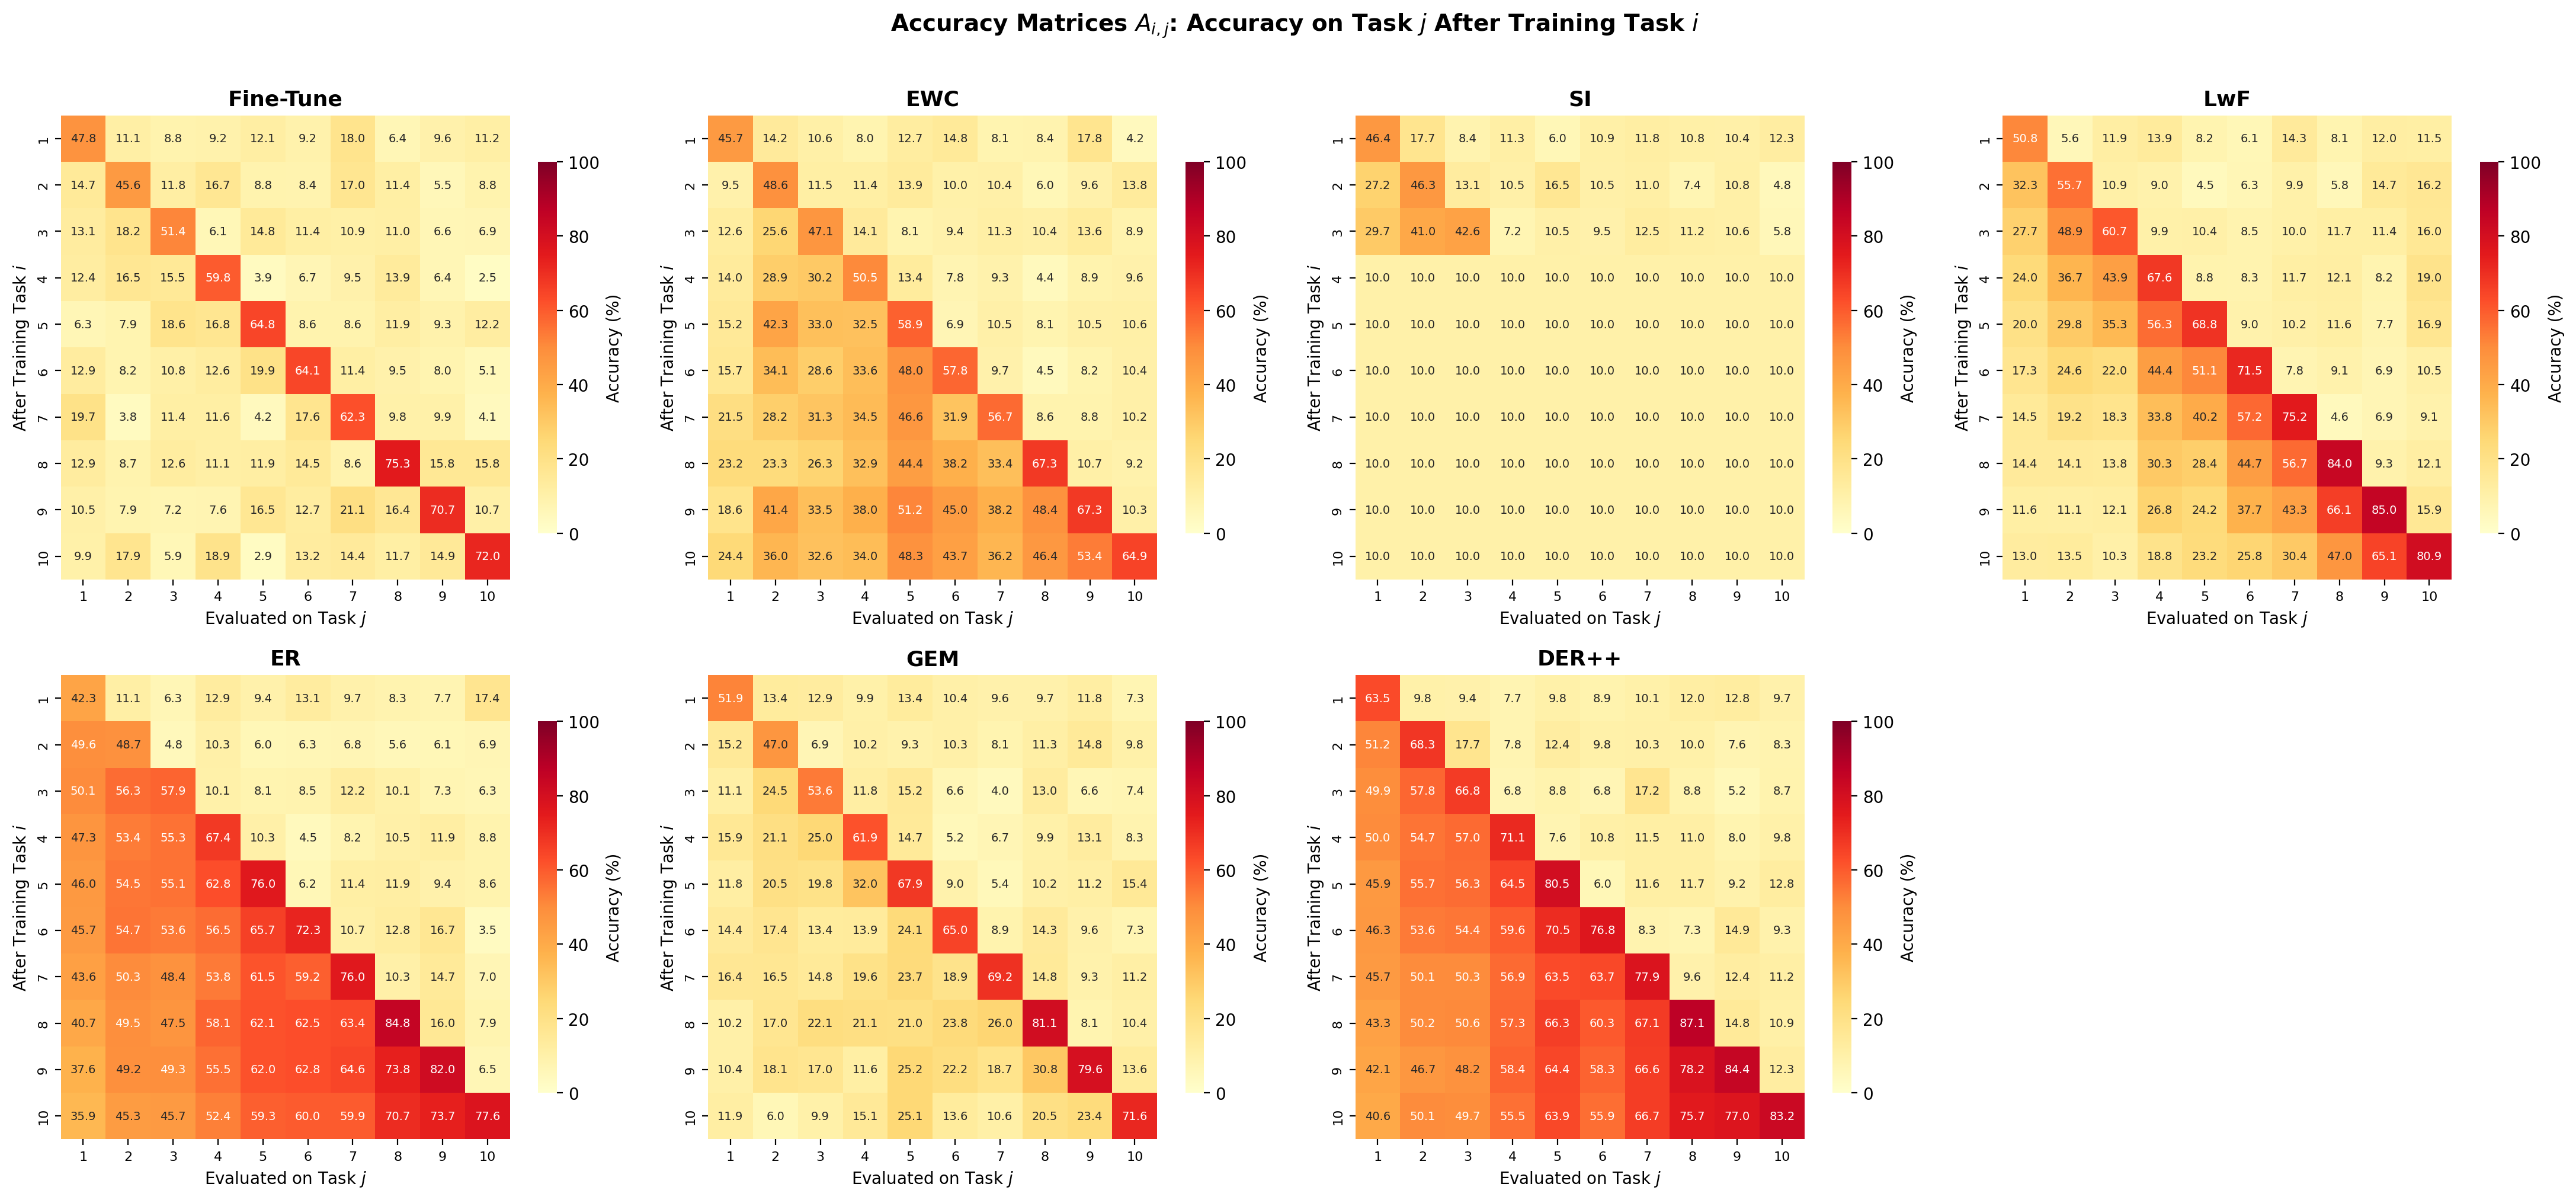
\includegraphics[width=\textwidth]{../accuracy_heatmaps.png}
\caption{Accuracy matrices $A_{i,j}$ for all seven methods. Colour scale fixed to $[0, 100]$. DER++ and ER maintain the highest off-diagonal accuracies; Fine-Tune and GEM exhibit severe forgetting.}
\label{fig:heatmaps}
\end{figure*}

\subsection{Metric Definitions}

We report four standard metrics from the accuracy matrix $A$:

\vspace{-6pt}
\begin{align}
  \bar{A} &= \tfrac{1}{K} \textstyle\sum_{j=1}^{K} A_{K,j} \label{eq:acc} \\[-1pt]
  \bar{F} &= \tfrac{1}{K{-}1} \textstyle\sum_{j=1}^{K-1} \bigl(\max_{i} A_{i,j} - A_{K,j}\bigr) \label{eq:forget} \\[-1pt]
  \mathrm{BWT} &= \tfrac{1}{K{-}1} \textstyle\sum_{j=1}^{K-1} (A_{K,j} - A_{j,j}) \label{eq:bwt} \\[-1pt]
  \mathrm{FWT} &= \tfrac{1}{K{-}1} \textstyle\sum_{j=2}^{K} (A_{j-1,j} - b_j) \label{eq:fwt}
\end{align}

\vspace{-4pt}
\noindent where $b_j = 10\%$ is the random baseline for 10-class tasks.

\subsection{Summary Table}

\begin{table}[H]
\centering
\caption{Quantitative comparison on Split CIFAR-100 ($K\!=\!10$). $\uparrow$/$\downarrow$ indicate desirable direction.}
\vspace{2pt}
\small
\begin{tabular}{l r r r r}
\toprule
\textbf{Method} & $\bar{A}\!\uparrow$ & $\bar{F}\!\downarrow$ & \textbf{BWT} & \textbf{FWT} \\
\midrule
Fine-Tune & 18.17 & 48.01 & $-48.01$ & $-0.09$ \\
EWC       & 42.00 & 16.10 & $-16.10$ & $+1.04$ \\
SI        & 10.00 & 13.17 & $-11.70$ & $+0.89$ \\
LwF       & 32.80 & 41.36 & $-41.36$ & $-0.91$ \\
ER        & 58.05 & 13.32 & $-11.61$ & $-0.44$ \\
GEM       & 20.77 & 49.01 & $-49.01$ & $+1.24$ \\
DER++     & \textbf{61.83} & \textbf{15.70} & $-15.70$ & $+0.32$ \\
\bottomrule
\end{tabular}
\label{tab:results}
\end{table}

% ══════════════════════════════════════════════════════════════════════════
\section{Analysis \& Discussion}

\textbf{Replay vs.\ regularization.}
ER ($\bar{A}\!=\!58.1\%$) and DER++ ($\bar{A}\!=\!61.8\%$) strongly outperform EWC ($42.0\%$) and LwF ($32.8\%$), confirming that 500 exemplars is more effective than parameter constraints. DER++ achieves the best result by combining replay with logit distillation ("dark knowledge").

\textbf{BWT and forgetting.}
Fine-Tune has BWT$\!=\!-48.0$ vs.\ EWC's $-16.1$ vs.\ ER's $-11.6$. EWC reduces forgetting $3\times$ via Fisher-weighted penalties. SI achieves low $\bar{F}\!=\!13.2$ but collapses to $\bar{A}\!=\!10\%$, indicating $c\!=\!1.0$ over-constrains learning.

\textbf{Surprising results.}
GEM ($\bar{A}\!=\!20.8\%$, BWT$\!=\!-49.0$) underperforms Fine-Tune---50 samples/task yields noisy reference gradients for A-GEM projection. LwF underperforms EWC as distillation degrades when CIFAR-100 subsets are dissimilar~\cite{li2016learning}. FWT$\approx 0$ for all methods, confirming minimal inter-task transfer.

\textbf{Limitations.}
(1)~Single seed; 3--5 runs recommended. (2)~Task-aware evaluation; class-incremental is harder. (3)~Shallow CNN; deeper models may alter rankings.

% ══════════════════════════════════════════════════════════════════════════
\section{Conclusion}

DER++ offers the best stability-plasticity trade-off ($\bar{A}\!=\!61.8\%$), combining replay with logit distillation. Replay-based methods consistently dominate regularization and distillation approaches on Split CIFAR-100~\cite{buzzega2020dark, delange2021survey}. Among non-replay methods, EWC provides the strongest forgetting reduction. A natural extension is to combine replay with regularization, or to evaluate under the harder class-incremental protocol.

% ══════════════════════════════════════════════════════════════════════════

\begin{thebibliography}{9}
\small

\bibitem{mccloskey1989catastrophic}
M.~McCloskey and N.~J.~Cohen, ``Catastrophic interference in connectionist networks: The sequential learning problem,'' \textit{Psychology of Learning and Motivation}, vol.~24, pp.~109--165, 1989.

\bibitem{kirkpatrick2017overcoming}
J.~Kirkpatrick et al., ``Overcoming catastrophic forgetting in neural networks,'' \textit{Proceedings of the National Academy of Sciences}, vol.~114, no.~13, pp.~3521--3526, 2017.

\bibitem{zenke2017continual}
F.~Zenke, B.~Poole, and S.~Ganguli, ``Continual learning through synaptic intelligence,'' in \textit{Proceedings of ICML}, 2017.

\bibitem{li2016learning}
Z.~Li and D.~Hoiem, ``Learning without forgetting,'' in \textit{Proceedings of ECCV}, pp.~614--629, 2016.

\bibitem{chaudhry2019continual}
A.~Chaudhry et al., ``Continual learning with tiny episodic memories,'' \textit{arXiv preprint arXiv:1902.10486}, 2019.

\bibitem{lopez2017gradient}
D.~Lopez-Paz and M.~Ranzato, ``Gradient episodic memory for continual learning,'' in \textit{Advances in NeurIPS}, 2017.

\bibitem{buzzega2020dark}
P.~Buzzega, M.~Boschini, A.~Porrello, D.~Abati, and S.~Calderara, ``Dark experience for general continual learning: A strong, simple baseline,'' in \textit{Advances in NeurIPS}, 2020.

\bibitem{delange2021survey}
M.~De~Lange et al., ``A continual learning survey: Defying forgetting in classification tasks,'' \textit{IEEE TPAMI}, 2021.

\end{thebibliography}

\end{document}
